\documentclass{scrartcl}
\usepackage{graphicx,tikz}
\usepackage{siunitx}
\usepackage[graphics,tightpage,active]{preview}
\newlength\imagewidth
\newlength\imagescale
\begin{document}
%%%%%%%%%%%%%%%%%%%%%%%%%%
\begin{preview}
	\newcommand{\imsize}{.333\linewidth}
	\pgfmathsetlength{\imagewidth}{\imsize} % desired display width of image
	\pgfmathsetlength{\imagescale}{\imagewidth/1024} % pixel width of image
	\def\size{1023}%
			%% Cutline between s1 and s2: 141 pixels %%
			%% Cutline between s2 and s3: 138 pixels %%
			\begin{tikzpicture}[x=\imagescale,y=-\imagescale]%
				\node[anchor=north west, inner sep=0pt, outer sep=0pt] at (0,0) {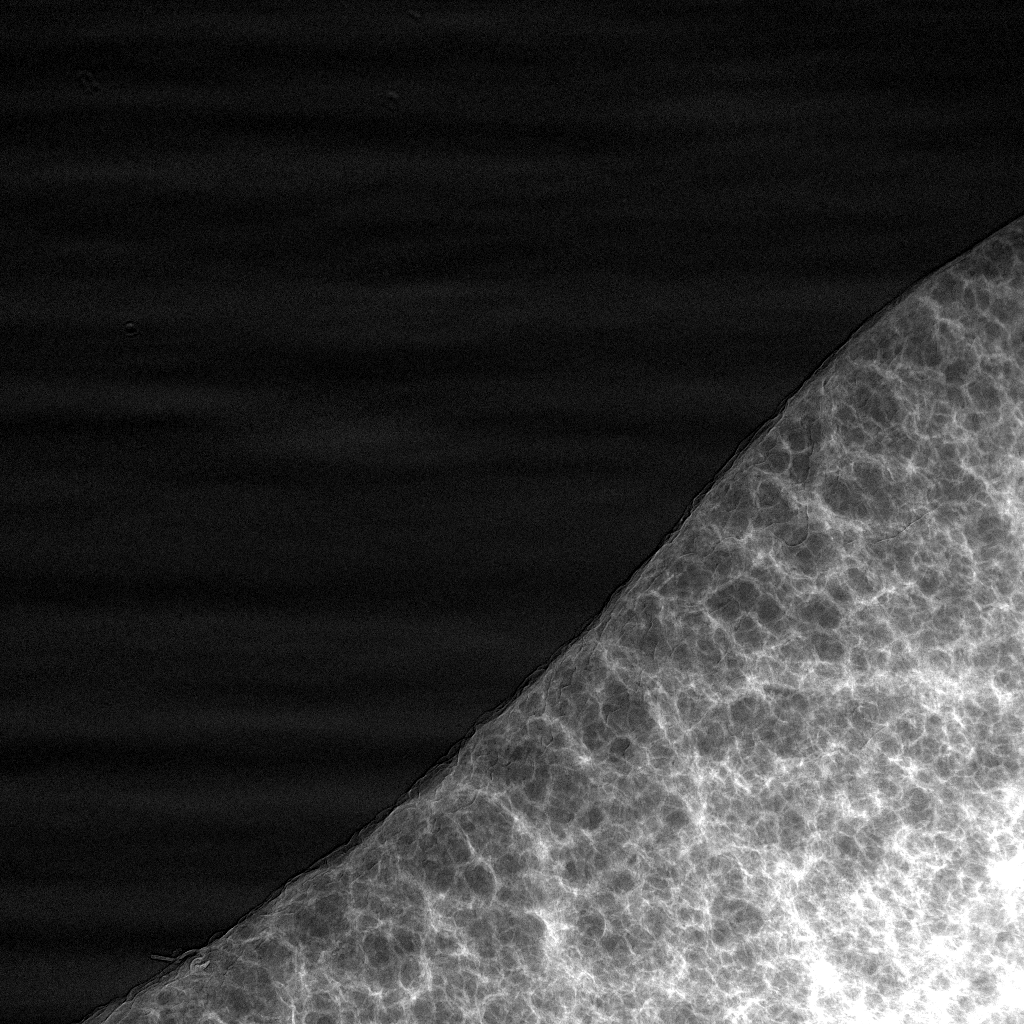
\includegraphics[width=\imagewidth]{../img/merge/CP-R108C21Cb_s13358_normalize}};%
				\def\overlap{141}%
				\fill [red, nearly transparent] (1024-\overlap,1) rectangle (\size,\size);%
				\draw (1024-\overlap,1) rectangle (\size,\size);%
				\node [anchor=south west, color=white] at (0,1024) {(a)};
			\end{tikzpicture}%
			\begin{tikzpicture}[x=\imagescale,y=-\imagescale]%
				\node[anchor=north west, inner sep=0pt, outer sep=0pt] at (0,0) {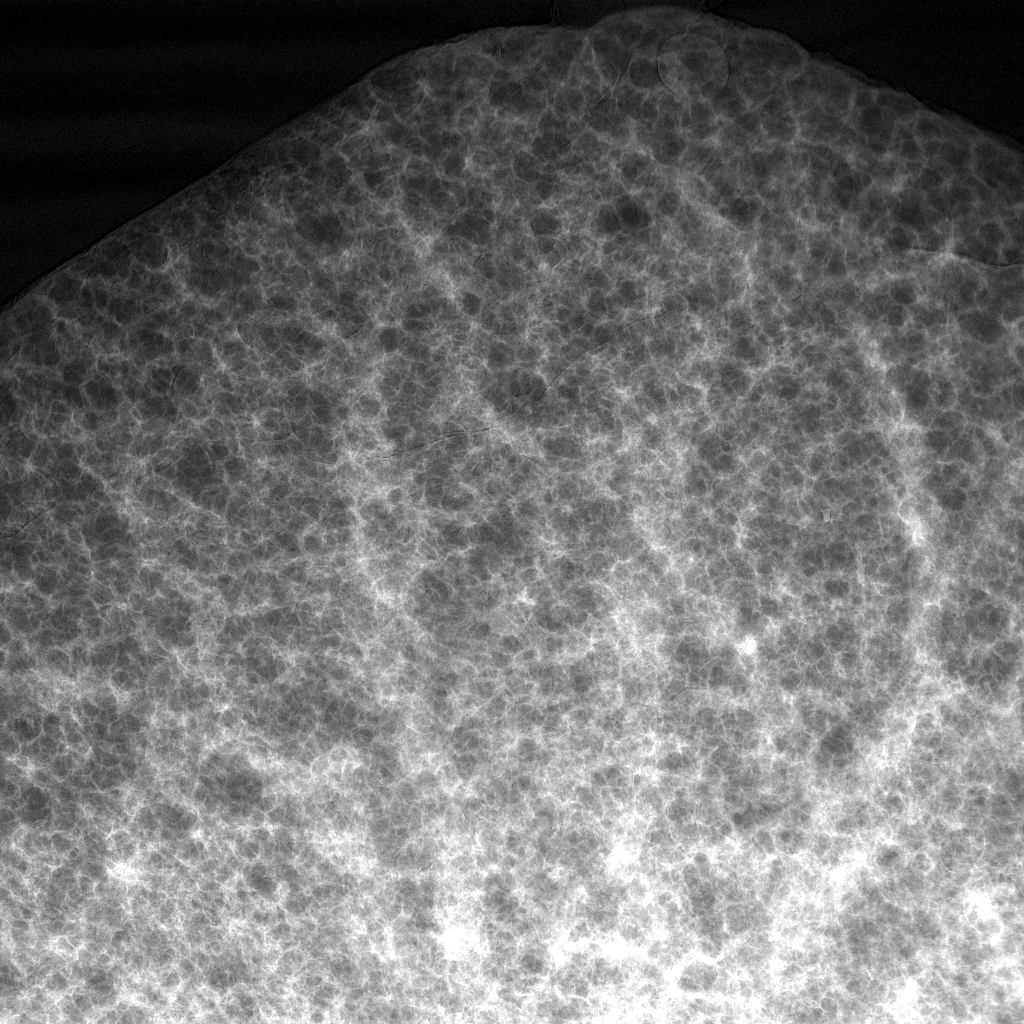
\includegraphics[width=\imagewidth]{../img/merge/CP-R108C21Cb_s23358_normalize}};%
				\def\overlap{141}%
				\fill [green, nearly transparent] (1,1) rectangle (\overlap,\size);%
				\draw (1,1) rectangle (\overlap,\size);%
				\def\overlap{138}%
				\fill [blue, nearly transparent] (1024-\overlap,1) rectangle (\size,\size);%
				\draw (1024-\overlap,1) rectangle (\size,\size);%
			\end{tikzpicture}%
			\begin{tikzpicture}[x=\imagescale,y=-\imagescale]%
				\node[anchor=north west, inner sep=0pt, outer sep=0pt] at (0,0) {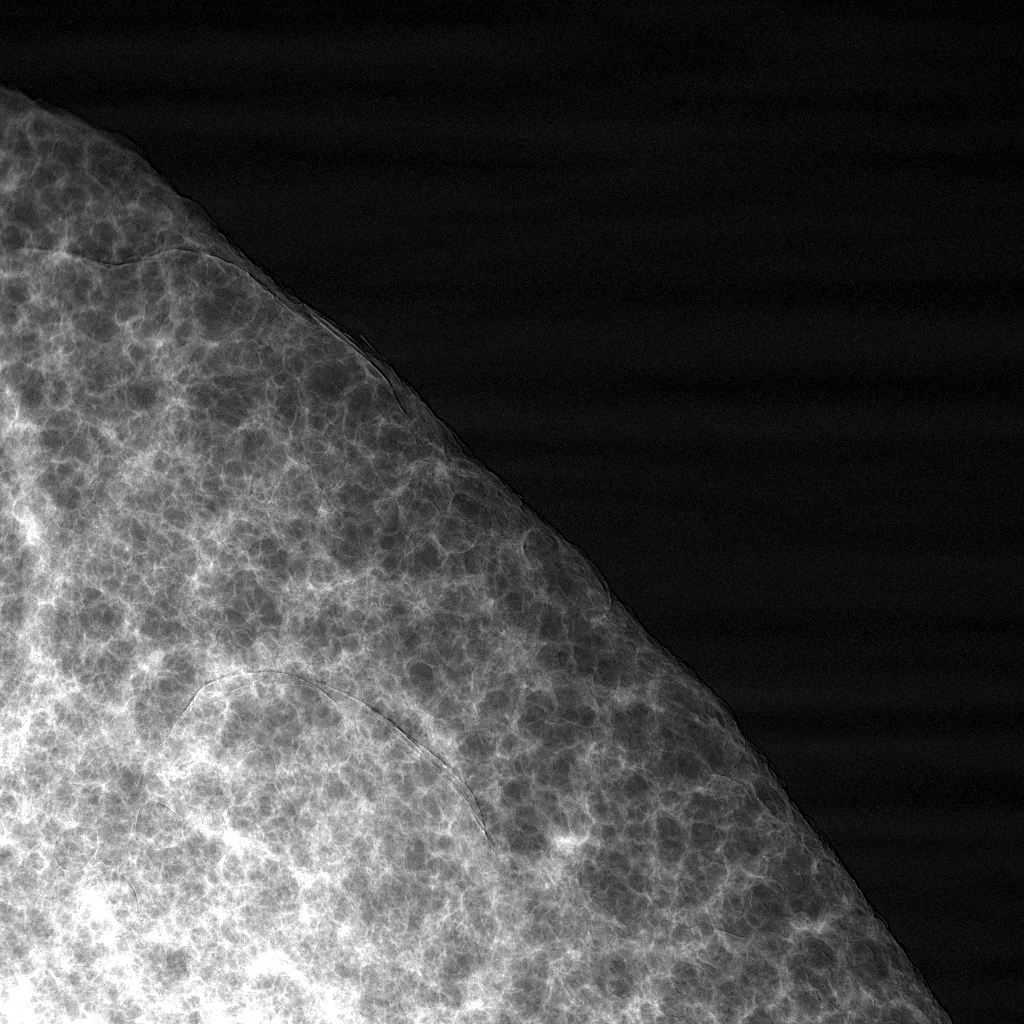
\includegraphics[width=\imagewidth]{../img/merge/CP-R108C21Cb_s33358_normalize}};%
				\def\overlap{138}%
				\fill [yellow, nearly transparent] (1,1) rectangle (\overlap,\size);%
				\draw (1,1) rectangle (\overlap,\size);%
				%\draw[|-|,thick] (5,200) -- (1021,200) node [color=white,midway,above] {\SI{1.51552}{\milli\meter}};%
				\def\x{924}% 1024 - 100
				\def\y{922}% 1024 * .9 = 921.6
				\def\bar{338}% 100 px = 148 um
				\draw[|-|,thick, color=white] (\x-\bar,\y) -- (\x,\y) node [midway, above] {\SI{500}{\micro\meter}};%
			\end{tikzpicture}%
	%%%%%%%%%%%%%%%%%%%%%%%%%%%%%%%%%%%
	\\
	%%%%%%%%%%%%%%%%%%%%%%%%%%%%%%%%%%%
	\renewcommand{\imsize}{\linewidth}%
	\pgfmathsetlength{\imagewidth}{\imsize} % desired displayed width of image
	\pgfmathsetlength{\imagescale}{\imagewidth/2793}% pixel width of image
		\begin{tikzpicture}[x=\imagescale,y=-\imagescale]%
			\node[anchor=north west, inner sep=0pt, outer sep=0pt] at (0,0) {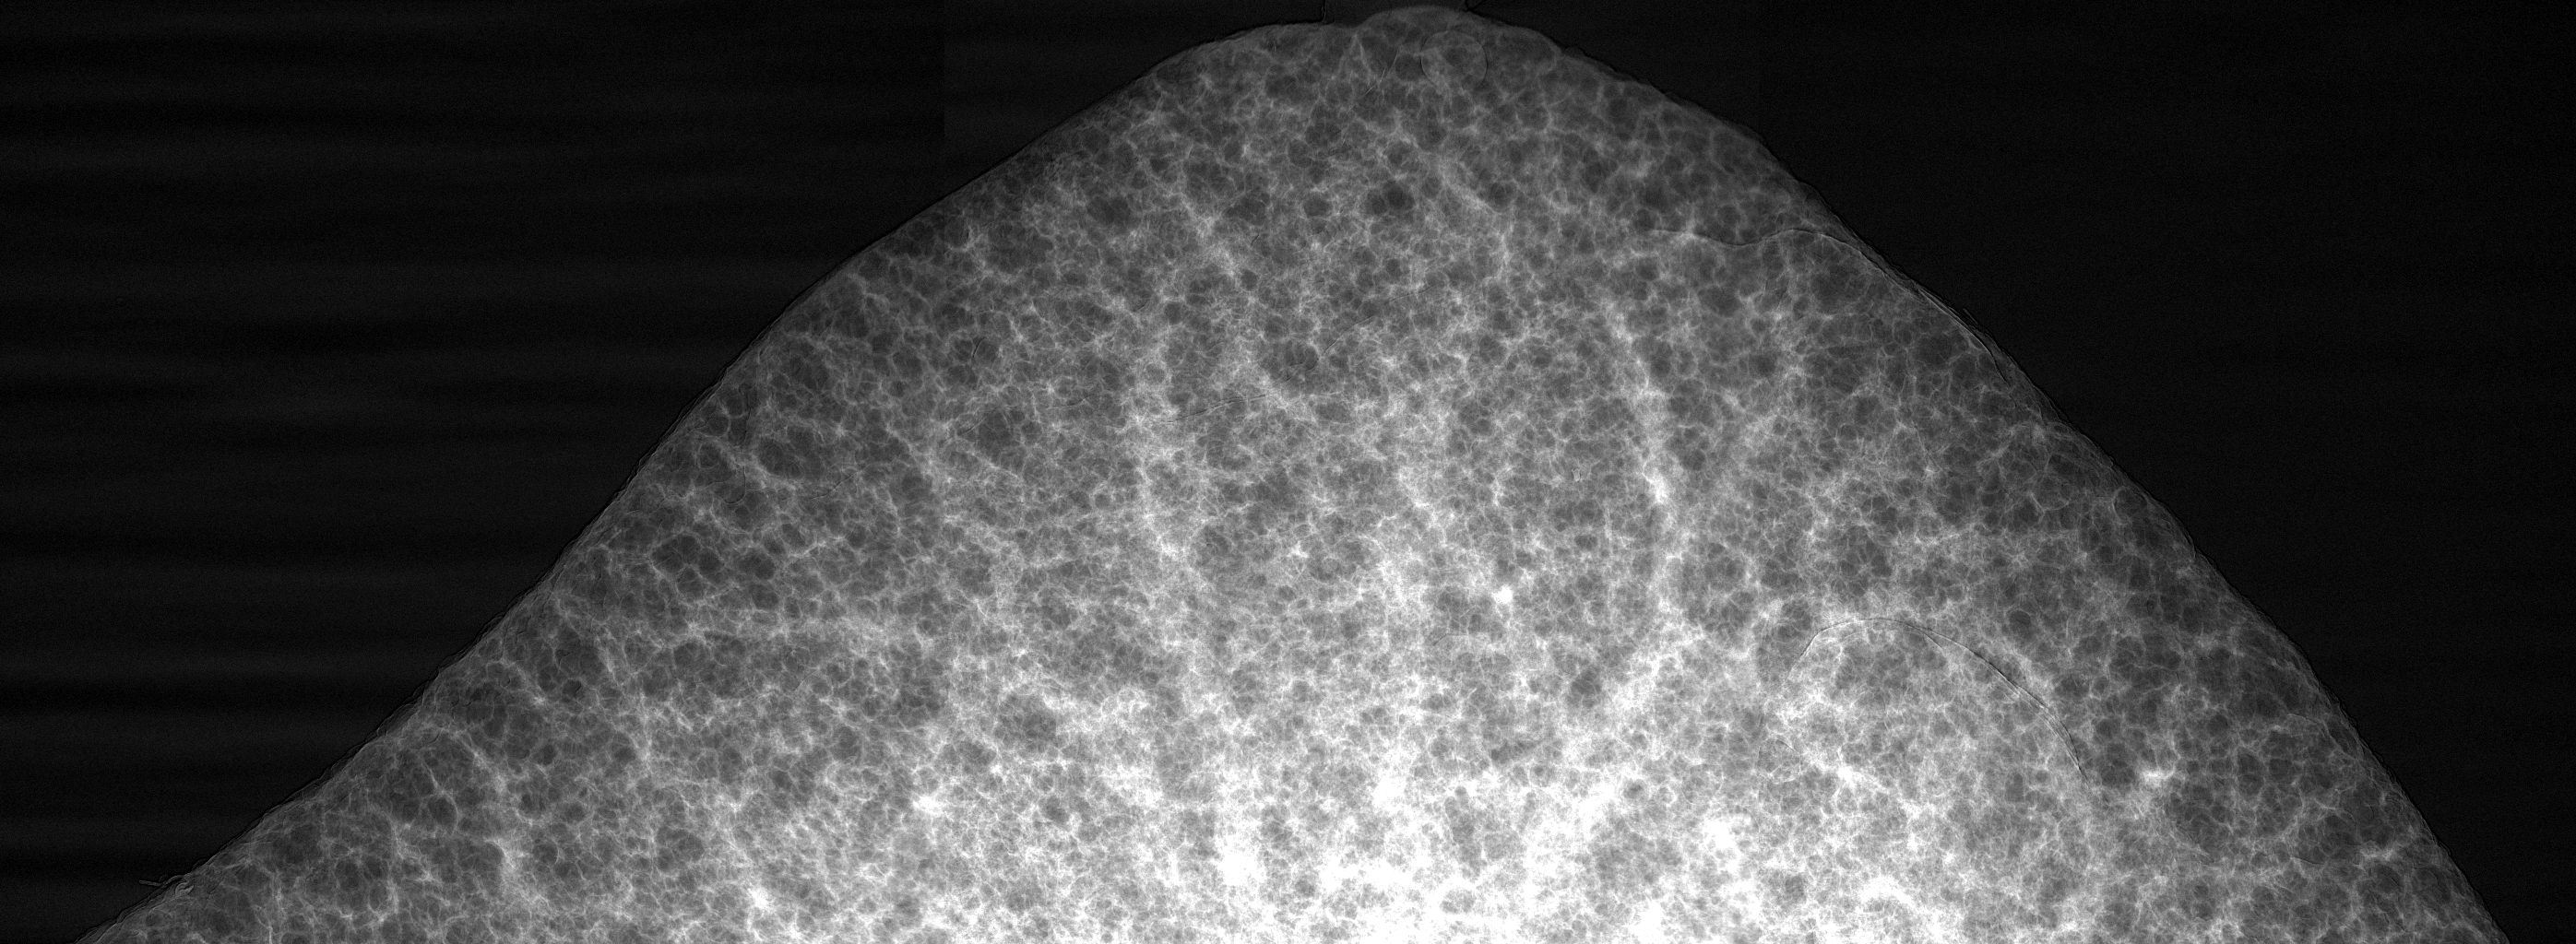
\includegraphics[width=\imagewidth]{../img/merge/R108C21Cb_mrg3333_normalize}};%
				\def\x{2693} % 2793-100
				\def\y{922} % 1024*.9 = 921.6
				\def\bar{338} % 100 px = 148 um
				%\draw[|-|,thick,color=white] (5,256) -- (2787,256) node [midway,above] {\SI{4.13364}{\milli\meter}};
				\draw[|-|,thick, color=white] (\x-\bar,\y) -- (\x,\y) node [midway, above] {\SI{500}{\micro\meter}};
				\node [anchor=south west, color=white] at (0,1024) {(b)};
				\end{tikzpicture}%
	%%%%%%%%%%%%%%%%%%%%%%%%%%%%%%%%%%%
	\\
	%%%%%%%%%%%%%%%%%%%%%%%%%%%%%%%%%%%
	\pgfmathsetlength{\imagewidth}{\imsize}%
	\pgfmathsetlength{\imagescale}{\imagewidth/2792}%
		\begin{tikzpicture}[x=\imagescale,y=-\imagescale]%
			\node [anchor=north west, inner sep=0pt, outer sep=0pt] at (0,0) {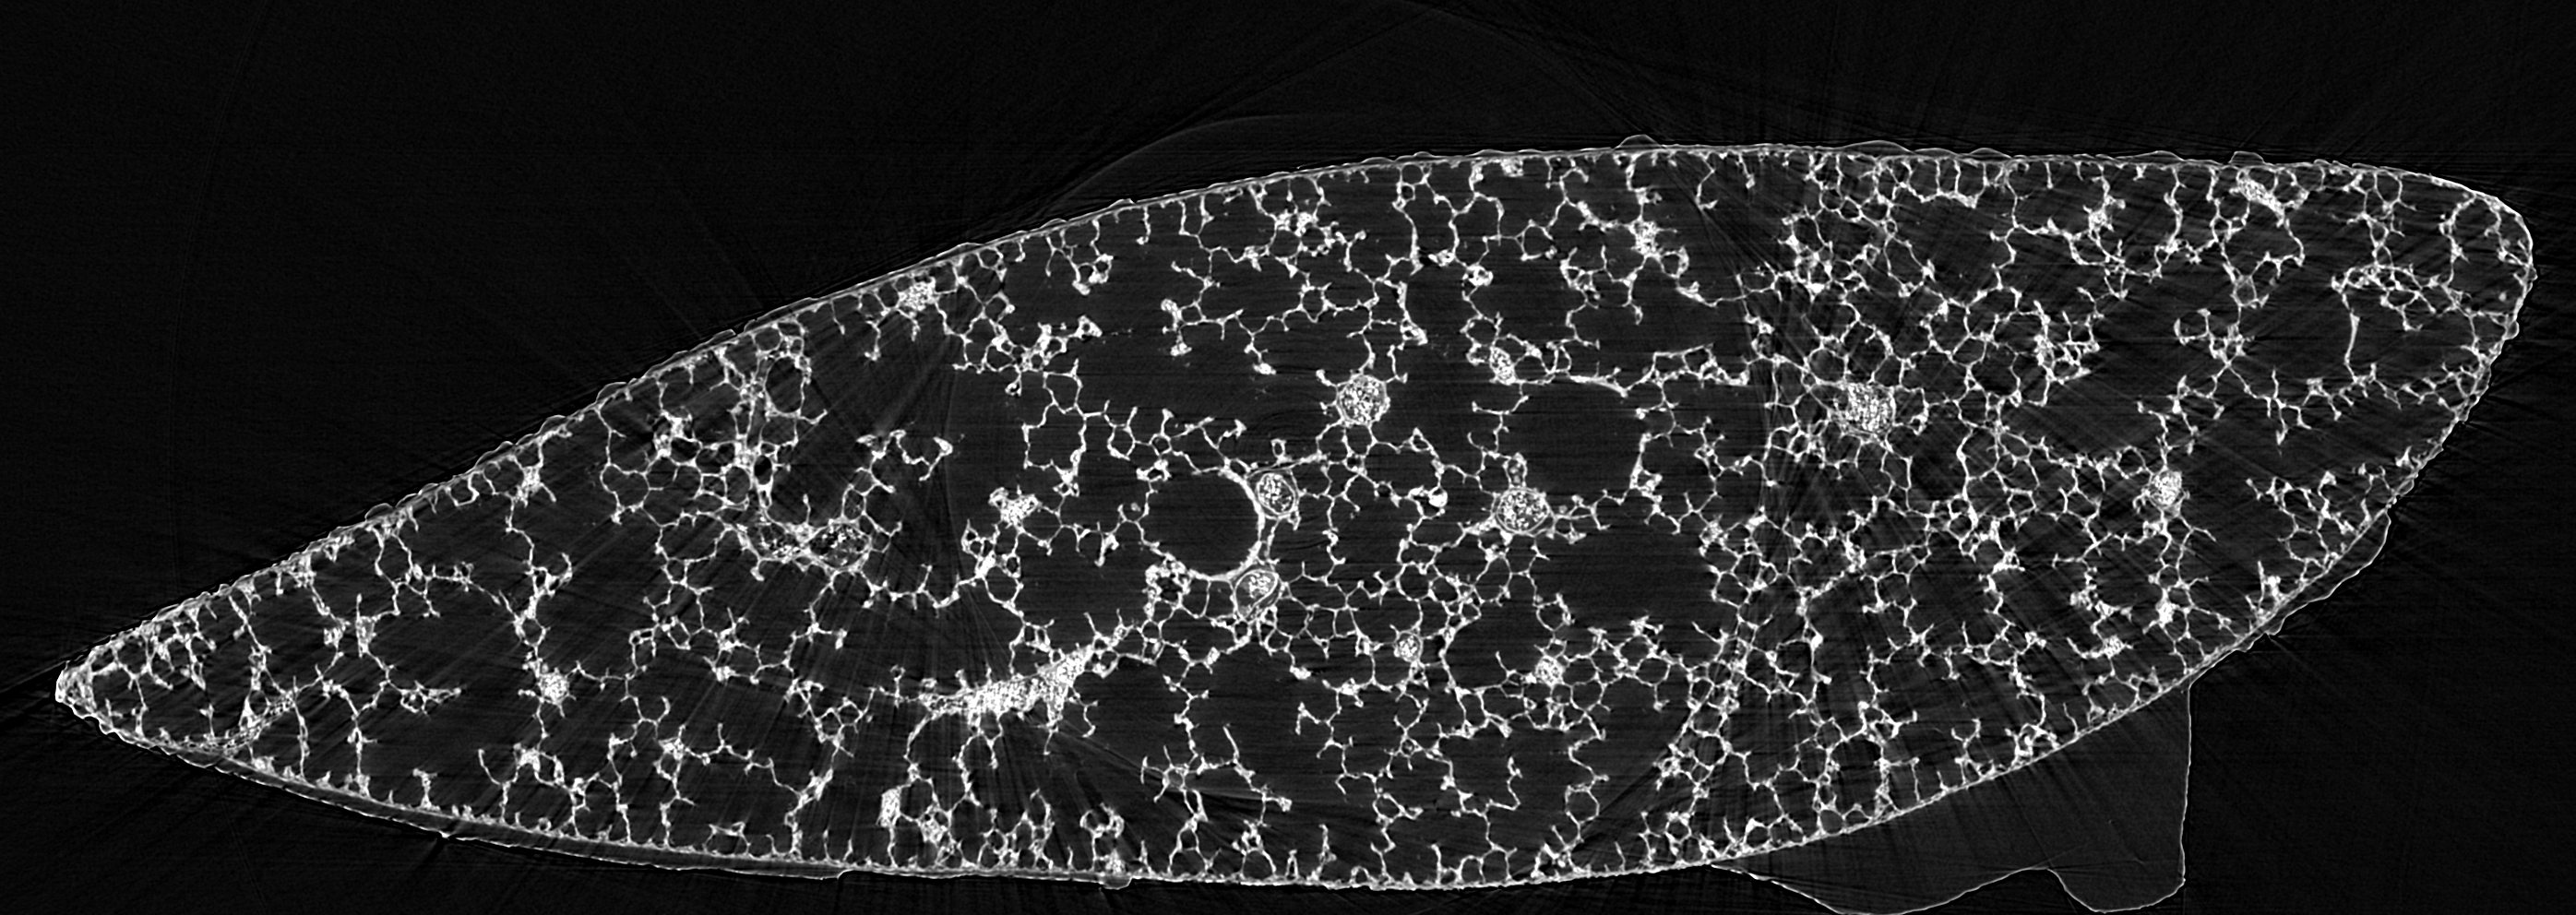
\includegraphics[width=\imagewidth]{../img/merge/R108C21Cb_mrg1024rec8bit}};
			\clip (0,0) rectangle (2792,992);				
			\def\x{2692} % 2792-100
			\def\y{893} % 992 * .9 = 892.8
			\def\bar{338} % 100 px = 148 um
			%%%% scalebar
				\draw[|-|,thick, color=white] (\x-\bar,\y) -- (\x,\y) node [midway, above] {\SI{500}{\micro\meter}};
				%\draw[|-|,thick, color=red] (5,30) -- (2787,30) node [midway, below] {\SI{4.13216}{\milli\meter}};
			%%%% big circle
				\draw [dashed, ultra thick, color=red] (2792/2,992/2) circle (512);
				\def\angle{35}
				\draw [white, thick, <->] (2792/2,992/2) +(\angle:0) -- node (bigto) {} +(\angle:512); 
				\node [white] (bigfrom) at (349,256){$\frac{1024}{2}$px};
				\draw [white, ->, thick, densely dotted] (bigfrom) to [bend left=45] (bigto);
			%%%% big circle
			%%%% 141px circle
			\draw [dashed, ultra thick, color=red] (2792/2,992/2) circle (512-141);
			\def\angle{35+90}
				\draw [white, thick,<->] (2792/2,992/2) +(\angle:0) -- node (smallto) {} +(\angle:512-141);
				\node [white] (smallfrom) at (349,384) {$\frac{1024}{2}-141$px};
				\draw [white, ->, thick, densely dotted] (smallfrom) to [bend left=45] (smallto);
			%%%% 141px circle					
			%%%% center
			\fill [color=red] (2792/2,992/2) circle (5);
			%%%% center
			\node [anchor=south west, color=white] at (0,990) {(c)};			
	%%%%%%%%%%%%%%%%%%%%%%%%%%%%%%%%%%%
	\end{tikzpicture}%
\end{preview}
%%%%%%%%%%%%%%%%%%%%%%%%%%
\end{document}